% This is based on the LLNCS.DEM the demonstration file of
% the LaTeX macro package from Springer-Verlag
% for Lecture Notes in Computer Science,
% version 2.4 for LaTeX2e as of 16. April 2010
%
% See http://www.springer.com/computer/lncs/lncs+authors?SGWID=0-40209-0-0-0
% for the full guidelines.
%
\documentclass{llncs}
\usepackage[utf8]{inputenc}
\usepackage[nolist,nohyperlinks]{acronym}

\begin{document}

\title{Power-Aware Security Protocols for the Internet of Things}
%
\titlerunning{}  % abbreviated title (for running head)
%                                     also used for the TOC unless
%                                     \toctitle is used
%
\author{Tiago Diogo}
%
\authorrunning{Tiago Diogo} % abbreviated author list (for running head)
%
%%%% list of authors for the TOC (use if author list has to be modified)
\tocauthor{Tiago Diogo}
%
\institute{Instituto Superior T\'ecnico, Avenida Rovisco Pais 1, Lisboa,\\
\email{tiago.diogo@tecnico.ulisboa.pt}}

\maketitle              % typeset the title of the contribution

\begin{abstract}
The abstract should summarize the contents of the paper
using at least 70 and at most 150 words.
\keywords{}
\end{abstract}

\section{Introduction}
\paragraph{}The \ac{IoT} can be seen as web of interconnected devices that go from everyday wearable objects into fully deployed sensor networks.Despite the huge variety and characteristics of these devices, one thing that they all have in common in the constrained nature they're built upon. In order to enable the massive deploy to be expected in the near future \footnote{http://blogs.wsj.com/cio/2015/06/02/internet-of-things-market-to-reach-1-7-trillion-by-2020-idc/} \ac{IoT} devices must be accessible and affordable, capable of operating under lossy wireless networks while being battery powered. This poses a challenge to current \ac{WWW} protocols since the assumptions regarding the devices capabilities and objectives do not hold true. To allow the \ac{IoT} vision to come forward, several new protocols have been developed across the OSI layers, each addressing and tackling the challenges involved in trying to keep the quality and assurances of stronger, more expensive protocols, on constrained systems. This document will address this issue from a power-aware perspective, meaning the battery consumption will be of major importance.


\section{Main Goals}
% Qual o objectivo e respectivos requisitos.
\paragraph{
Given the constraints and limitations of \ac{IoT} devices described in the previous chapter, the first objective of this work is to identify existing protocols at the OSI application layer that take into account those constrains and are design to allow communication between these devices without consuming an amount of resources that would be appropriate for standard devices but excessive for the \ac{IoT} ones.
}

\paragraph{
After the analysis of the existing solutions, a baseline of power consumption will be established. Then, the focus will move towards adding confidentiality to the transmitted information by securing the channel.
Once both the application level protocols and proper security solutions are defined, experiments will be performed so that the added power consumption cost of adding the security layers can be measured, profiled and documented therefore enabling the finding of the best parameters for a desired level of security.
}

\paragraph{
The work will then proceed towards finding effective counter-measures against a specific group of attacks that targets the \ac{IoT} devices by intensifying the use of its resources therefore draining the available power and placing the node offline.
The ultimate goal is to propose an energy-efficient security mechanism that can resist these power-drain (a.k.a vampire) attacks.
}

\section{Related Work}
\subsection{Protocol Analysis and Selection}
\label{sec:protocol_analysis}

\paragraph{}
There are many alternatives and some proposed standards when it comes to choosing a protocol stack for \ac{IoT} communications. The decision must be based on the particularities of the devices to be used and the objective of the application itself, however a thoroughly analysis of the existing solutions is a proper way to unveil the strong and weak points of each protocol providing a good basis for an informed decision. A recent survey (January 2015) \cite{Al-Fuqaha2015} of the \ac{IoT} enabling technologies, protocols and applications will be the starting point for the analysis to follow. The presentation of the available protocols and solutions will follow a bottom-up approach, starting from the data link and physical layer all the way up until the application layer. In particular, the session layer will be left to the end since securing the channel is an optional feature and will be addressed after the application level protocols are properly examined.

\subsubsection{Data Link and Physical Layer}

\paragraph{}
The first requirement for the physical layer of the \ac{IoT} is the use of wireless radios. These should aim for simplicity, low-power and low-cost communications. While wireless communication are far spread and can be found from homes to airports, the type of radio commonly used, known as Wi-Fi, use a high amount of power causing concerns for battery life. In the next paragraphs, an overview of Wi-Fi(IEEE 802.11) is given with the objective of comparing it with the IEEE 802.15.4, a protocol that aims to address these issues.

\paragraph{\textbf{IEEE 802.11}}
\paragraph{}
IEEE 802.11 is a set of standards for \ac{WLAN} communications. They are the basis for the so called Wi-Fi. IEEE 802.11 is concerned with Ethernet matching speed, long ranges, message forwarding and high data throughput. These concerns directly clash with the \ac{IoT} objectives and account for the added power consumption of this protocol.

\paragraph{\textbf{IEEE 802.15.4}}
\paragraph{}
IEEE 802.15.4 on the other hand was created for \ac{LR-WPAN} and its specifications on low power consumption, low data rate, low cost and high message throughput make it a strong candidate for \ac{IoT} applications.
	The IEEE 802.15.4 standard supports two types of network nodes, the \ac{FFD} that act as coordinator or normal nodes. And the \ac{RFD} that are very simple, with very restricted resources and can only communicate with coordinators. The coordinators are responsible for controlling and maintaining the network. \ac{FFD} are capable of storing a routing table in their memory and can implement a full \ac{MAC}.
	IEEE 802.15.4 supports star, peer-to-peer(mesh) and cluster-tree topologies.
	Regarding performance, it would be unfair to directly compare the two, since IEEE 802.11 transmission power and receiver sensitivity and much greater than 802.15.4. But if we limit both to a low power level IEEE 802.11 still outperforms IEEE 802.15.4 in terms of packet delivery ratio, throughput, latency, jitter and and average energy consumption. However this comes at the cost of a far lower transmission range\cite{Transmission2011}.
	We can conclude that for typical \ac{LR-WPAN} network requirements, IEEE 802.15.4 is better designed to address the constrained environment issues, while IEEE 802.11 would still be a suitable option if transmission range is not a problem.

\subsubsection{Network Layer}
\label{sec:network_layer}

\paragraph{\textbf{6LoWPAN}}
\paragraph{}
	The \ac{IoT} vision, as presented in the introduction, and its massive deployment can only be achieved through the use of IPv6. However, physical layers more suitable for communication over constrained networks pose some limitations to the use of the IPv6 messages. For example the limited packet size in IEEE 802.15.4 based networks. To tackle these issues, the \ac{IETF} 6LoWPAN working group developed a standard based on header compression to reduce the transmission overhead, fragmentation to meet the IPv6 \ac{MTU} requirements and forwarding to link-layer to support multi-hop delivery. \cite{Hui2008}
	6LoWPAN is able to remove a major share of IPv6 overheads, being able to compress its headers to two bytes, therefore allowing small IPv6 datagrams to be sent over IEEE 802.15.4 networks. 
	
\paragraph{\textbf{RPL}}
\paragraph{}
With the use of 6LoWPAN, upper layer routing protocols can now use the IPv6 addressing scheme. Given the possible frequent topology changes associated with the radio-link instability, successful  solutions must take these requirements into account on their specification. RPL can support a wide variety of link-layers and is prepared for devices with very limited resources. It is able to build up network routes, distribute routing knowledge among nodes and adapt the topology in a very efficient way. More in depth, RPL creates a \ac{DODAG} between the 6LoWPAN network nodes (Figure \ref{fig:rpl_dodag}) that supports unidirectional traffic towards the \ac{DODAG} root and bidirectional traffic between devices. Each node has a rank that indicates it's position relative to other nodes and with respect to the root. This rank is used to create optimized network paths. In order to allow packets to propagate downwards the the topology, either source routing or stateful routing tables are used. (More Information on this two types of routing are given in sections \ref{sec:source_routing} and \ref{sec:tables_routing}). For both modes, the \ac{DODAG} root always maintains a complete list of the network nodes. RPL provides a set of control messages in order to exchange routing graph information. \ac{DIO} are used to advertise information needed to build the \ac{DODAG}. \ac{DAO}  are used to advertise information so that downwards traffic can go through the nodes towards the leafs. Nodes may also resort to \ac{DIS} messages to request graph information from neighbour nodes. Finally, RPL has a built in topology repair mechanism that acts in the case of a routing topology failure, link failure or node failure. In the case the topology needs to be rebuilt, a link layer metric is used to calculate the new route. The new path is considered fit for work if the link layer acknowledgements are received on it.

\begin{figure}[h]
  \centering
  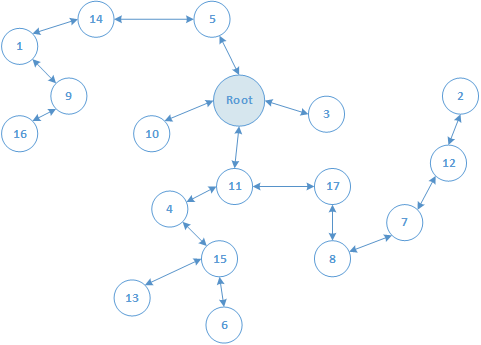
\includegraphics[width=0.8\linewidth]{figures/RPL_DODAG.png}
  \caption{A Sample RPL DODAG}
  \label{fig:rpl_dodag}
\end{figure}

\subsubsection{Application Layer}

\paragraph{\textbf{\ac{HTTP}}}
\paragraph{}
	\ac{HTTP} is an application level protocol that works in the request-response model and is the foundation of data communication on the \ac{WWW} It is primarily designed to run over \ac{TCP} which is a problem in lossy and constrained environments due to the delivery assurances and congestion control algorithms it employs. Besides, {HTTP} is verbose, text-based, and not suited for compact message exchanges. Moreover, the header size required for a message exchange can leave too few payload space in constrained networks like the IEEE 802.15.4-based networks where the \ac{MTU} size of the protocol is 127 bytes. These protocol specifications would not raise any issues in standard \ac{WWW} communications, but when it comes to constrained environments it is clear that the protocol is not adequate to the necessities of \ac{IoT} devices and networks.

\paragraph{\textbf{\ac{CoAP}}}
\paragraph{}
	\ac{CoAP} is a document transfer protocol based on \ac{REST} on top of \ac{HTTP} functionalities. \ac{CoAP} objective is to enable tiny constrained devices to use RESTful interactions, where clients and servers expose and consume web services using \ac{URIs} together with  \ac{HTTP} get, post, put and delete methods. Unlike \ac{REST}, \ac{CoAP} runs over \ac{UDP} instead of \ac{TCP} which makes it suitable for full IP networking in small micro-controllers. Retries and reordering are implemented at the application stack using a messaging sub-layer that detects duplicated messages and provides reliable communication using different types of messages. Confirmable messages must be acknowledged by the receiver, nonconfirmable follow the fire and forget model. While being a lightweight protocol, \ac{CoAP} still provides important features:
	
\begin{itemize}
	\item Resource Observation - \ac{CoAP} can extend the \ac{HTTP} request model with the ability to observe a resource therefore monitoring resources of interest using a publish/subscribe mechanism.\\
	\item Resource Discovery - \ac{CoAP} servers provide a list of resources using well-known {URIs} that allow clients to discover what resources are provided and their types.\\
	\item Interoperability - since \ac{CoAP} is based on the \ac{REST} architecture, a simple proxy enables \ac{CoAP} to easily interoperate with \ac{HTTP}.
\end{itemize}

\paragraph{}
A study that compared \ac{CoAP} and \ac{HTTP} using mobile networks concluded that there is no situation where \ac{CoAP} would consume more resources than \ac{HTTP} \cite{Savolainen2014}

\paragraph{\textbf{\ac{MQTT}}}
\paragraph{}
	\ac{MQTT} is a publish/subscribe messaging protocol designed for lightweight \ac{M2M} communications. It employs a client/server model and consists of three components, the publisher, the subscriber and a broker.
Subscribers register their interest for a specific topic and then get informed by the broker when a publisher generates data regarding that topic. Every message is a discrete chunk of data, opaque to the broker. The broker, on is side, checks authorization of the publishers and subscribers. \ac{MQTT} supports three Application Level \ac{QoS} levels:

\begin{itemize}
	\item At Most Once (Fire and Forget): A message will not be acknowledged by the receiver or stored and redelivered by the sender.\\
	\item At Least Once: It is guaranteed that the message will be delivered to the receiver, but more that one can reach the destination due to message resending. The sender stores the message until it gets an acknowledge from the receiver.\\
	\item Exactly Once: A four-way handshake mechanism is used to guarantee that the message will be received exactly once by the counterpart.
\end{itemize}

\paragraph{}
\ac{MQTT} has support for persistent messages stored on the broker, where the most recent message will be sent to a client that subscribes that topic. Clients can register a custom message to be sent to the broker on disconnect enabling other subscribers to know when a device disconnects. \ac{MQTT} runs on \ac{TCP} which in some cases causes drawbacks in performance. A performance evaluation of \ac{MQTT} and \ac{CoAP} \cite{Ma2014} provides comparisons on several protocol facets:

\begin{itemize}
	\item Influence of Packet Loss on Delay: With low values of packet loss, \ac{MQTT} experienced lower delays, but as the packet loss increased \ac{CoAP} performed better. This is due to the greater \ac{TCP} overheads involved in the retransmissions of messages when compared to \ac{UDP}.\\
	\item Influence of Packet Loss on Data Transfer: \ac{CoAP} generated less data for each packet loss versus all the \ac{MQTT} \ac{QoS} levels.\\
	\item Overheads for Message Sizes: When packet loss rate is low, \ac{CoAP} generates less overhead than \ac{MQTT} for all message sizes, but as message size grows, the reverse is true. This happens because when the message size is is large, the probability that \ac{UDP} loses the message is higher than \ac{TCP} which causes \ac{CoAP} to retransmit the whole message more often than \ac{MQTT}.
\end{itemize}

\paragraph{}
	In order to address the drawbacks on constrained devices, \ac{MQTT-SN} protocol\cite{Ibm2013} was created. Among the improvements and new features, \ac{MQTT-SN} runs on UDP, adds broker support for indexing topic names, provides a discovery procedure to help clients without a pre-configured server address and supports devices in sleep state. With this approach, an extra gateway is necessary to convert from \ac{MQTT-SN} to \ac{MQTT} so the communications can be understand by the broker.

\subsubsection{Session Layer}

\paragraph{}
So far security issues have not been address in any of the previous layers, this is because security is an expensive, optional feature. The application layer protocols rely on underneath layers to achieve secure communications, and network layer protocols assume that if security in necessary then it has already been handled in upper layer protocols. In fact, the session layer is where the security mechanisms are implemented and provides an abstraction layer to application layer protocols. These mechanisms work on top of the transport layer and aim to provide authentication, confidentiality and message integrity.

\paragraph{\textbf{\ac{TLS}}}
\paragraph{}
	\ac{TLS} is a well-known security protocol that is used to provide secure transport layer for \ac{TCP} communications, allowing the upper layer protocols to be left untouched. \ac{TLS} operation consists of two phases: the handshake and then the data encryption. During the handshake, both parties negotiate which algorithms will be used during the session, authenticate themselves, and prepare the shared secret for the data encryption.
	Both \ac{HTTP} and \ac{MQTT} work over \ac{TCP} and use \ac{TLS} as the adopted security protocol.

\paragraph{\textbf{\ac{DTLS}}}
\paragraph{}
	\ac{DTLS} aims to be the equivalent of \ac{TLS} over \ac{UDP} transport layer. \ac{DTLS} works over datagrams that can be lost, duplicated, or received in the wrong order, therefore needing some extra mechanisms(application layer protocols \ac{QoS}) to cope with that. Although both \ac{CoAP} and \ac{MQTT-SN} work over \ac{UDP} and use \ac{DTLS} as the adopted security, some authors argue that \ac{DTLS} is not a suitable option \cite{Alghamdi2013} and defend the need of a new integrated security solution. Some of the presented drawbacks are:

\begin{itemize}
	\item There is no multicast support, which is a key feature in \ac{IoT} (topology discovery and update for example).
	\item Handshake phase is prone to exhaustion attacks on the device resources.
	\item The loss of a message in-flight requires the retransmission of all the messages in-flight.
\end{itemize}

\paragraph{}
	A final overview of the analysed protocols and security solutions is given in Table \ref{tab:protocols}. And a comparison of the protocol stack is shown in Table \ref{tab:stack}. 

\begin{table}[h]
	\centering
	\begin{center} \caption{\ac{IoT} Application Protocols Comparison} \label{tab:protocols} \end{center}
	\begin{tabular}{c|cccccc}
		\begin{turn}{90}\begin{tabular}{@{}c@{}}Application \\ Protocol\end{tabular}\end{turn} &
		\begin{turn}{90}RESTful\end{turn} &
		\begin{turn}{90}\begin{tabular}{@{}c@{}}Request/ \\ Response\end{tabular}\end{turn} &
		\begin{turn}{90}\begin{tabular}{@{}c@{}}Publish/ \\ Subscribe\end{tabular}\end{turn} &
		\begin{turn}{90}Adjustable \ac{QoS}\end{turn} &
		\begin{turn}{90}Transport\end{turn} &
		\begin{turn}{90}Security\end{turn} \\
		\hline
		\ac{HTTP} & \hspace{0.2cm}\cmark\hspace{0.2cm} & \hspace{0.2cm}\cmark\hspace{0.2cm} &
		 \hspace{0.2cm}\xmark\hspace{0.2cm} & \hspace{0.2cm}\xmark\hspace{0.2cm} & 
		 \hspace{0.2cm}\ac{TCP}\hspace{0.2cm} & \hspace{0.2cm}\ac{TLS}\hspace{0.2cm} \\
		%\hline
		\ac{CoAP} & \cmark & \cmark & \cmark & \cmark & \ac{UDP} & \ac{DTLS} \\
		%\hline
		\ac{MQTT} & \xmark & \xmark & \cmark & \cmark & \ac{TCP} & \ac{TLS}\\
		%\hline
		\ac{MQTT-SN} & \xmark & \xmark & \cmark & \cmark & \ac{UDP} & \ac{DTLS}
	\end{tabular}
\end{table}


\begin{table}[h]
	\centering
	\begin{center} \caption{Protocol Stack Comparison Overview } \label{tab:stack}\end{center}
	\begin{tabular}{c|c|c}
		Layer & Web & IoT \\
		\hline
		Application & \ac{HTTP} & \ac{CoAP} \\
		Session & \ac{TLS} & \ac{DTLS} \\
		Transport & \ac{TCP} & \ac{UDP} \\
		Network & IPv6 & 6LoWPAN \\
		Data-Link/Phy & 802.11 & 802.15.4
	\end{tabular}
\end{table}

\subsection{Attack Analysis, Detection and Mitigation}
\label{sec:attack_analysis}
\paragraph{}
Exploitation of existing solutions in the forms of malicious attacks can be found at all the studied OSI layers. They can go from the well-known \ac{DoS} at the application layer to a physical intruder replacing some node on a sensor field. However, given the characteristics of the devices and networks used in \ac{IoT} combined with the power consumption focus of this work, a specific kind of attacks performed at the network layer is of special interest and importance:

\paragraph{\textbf{Battery Depletion Attacks aka Vampire Attacks}}
\paragraph{}
Battery Depletion Attacks aim at draining the battery, "life", of the network devices, working over time to entirely disable a network, hence being called Vampire Attacks. These attacks do not focus on flooding the network with many packages, instead they drain the node's life by delaying the packets transmission. Many of the existing attacks are not protocol specific \cite{Vasserman2013}, while others target specific protocols and implementations \cite{Pongle2015}. The following attacks aim at giving an overview of the existing attack possibilities on different routing solutions as well as existing mitigation strategies. Additionally, a range of attacks that target the RPL routing protocol is also analysed. Since RPL is the selected protocol of our energy efficient stack, it is of special importance to consider and assure the mitigation of attacks that would drain the devices batteries by exploiting this light weight protocol inner workings.   

\subsubsection{Stateless Protocols}
\label{sec:source_routing}
\paragraph{}
In systems that use this type of routing protocols, the source node specifies the entire route to the destination in the packet header. This means that intermediaries do not make decisions regarding the next hop, they only forward to the next node as specified in the original path therefore reducing the amount of computation performed and used energy. However, the source node must ensure that the route is valid at the time of sending and that the neighbour relations among the devices allow the specified forwarding path. Using this transmission scheme, a malicious device can specify paths through the network that are far from optimal, wasting energy at the intermediate nodes who follow the included malicious source route. A couple examples of these attacks are the Carousel and Stretch Attacks.

\paragraph{\textbf{Carousel Attack}}
\paragraph{}
The objective of this attack is to send a packet along a route composed as a series of loops. This way a single node may forward the malicious packet several times increasing the total energy consumption by a factor of the number of loops the attacker has introduced on the packet header path. It targets source routing protocols by exploiting the limited verification of the packets headers at the intermediary nodes. Figure \ref{fig:carousel_attack} shows an example where a vampire node created a path composed of circles around the network when it could exit after the first hop through the D node.
 
\begin{figure}[h]
  \centering
  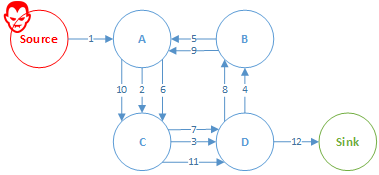
\includegraphics[width=0.8\linewidth]{figures/Carousel_Attack.png}
  \caption{Carousel Attack}
  \label{fig:carousel_attack}
\end{figure}

Existing mitigations strategies rely on checking the source route for loops on intermediary nodes, either selecting an appropriate route for the packet or simply dropping it.

\paragraph{\textbf{Stretch Attack}}
\paragraph{}
The objective of this attack is to create a longer source route around the network than the one who would be required to transverse the network from the source to the sink. The number of elements in the path would be greater than the optimal path, therefore increasing the total energy consumption by a factor of the number of additional hops. It's success rests on intermediary nodes not checking for better paths. Figure \ref{fig:stretch_attack} shows an example where a vampire node created a path that goes through a greater number of nodes than required to reach the sink.

\begin{figure}[h]
  \centering
  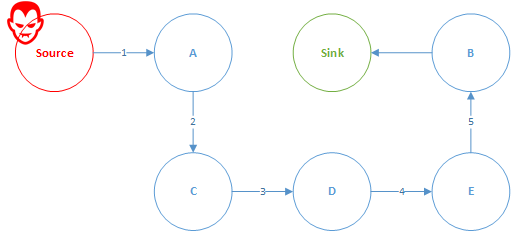
\includegraphics[width=0.8\linewidth]{figures/Stretch_Attack.png}
  \caption{Stretch Attack}
  \label{fig:stretch_attack}
\end{figure}

A limited way of mitigating this attack would be to ensure that path routes have less than the total number on devices on the network. Vasserman and Hoper proposed a property called "no-backtracking" that assures the packet is always moving closer to the sink on every hop. \cite{Vasserman2013}

\subsubsection{Stateful Protocols}
\label{sec:tables_routing}
\paragraph{}
In systems that use this type of routing protocols, network nodes are aware of the network topology and it's state, being able to make local decisions on the node to whom they will forward the packet. The effect of the Vampires on this type of routing is limited since the route is built dynamically from many independent forwarding decisions. However, attackers can still cause damage by forcing packet forwarding through nodes that would not be on the optimal path, for example by forwarding the packet back to the source. A couple examples of these attacks are the Directional Antenna and Wormhole Attacks.

\paragraph{\textbf{Directional Antenna Attack}}
\paragraph{}
In this attack, the attacker takes the role of an intermediary and not the source of a packet. If the attacker has the resources to use a directional antenna, it can deposit a packet on arbitrary parts of the network while also forwarding the packet locally. This causes nodes that were not on the optimal path to also consume energy by forwarding a packet they would not normally receive, therefore increasing the total energy consumption by a factor of the directions the attacker can position the antenna and the distance between the receiver and the sink. Figure \ref{fig:directional_antenna_attack} shows an example where a vampire intermediary deposited a node on a distant location of the network, causing the packet to follow 2 different routes towards it's destination

\begin{figure}[h]
  \centering
  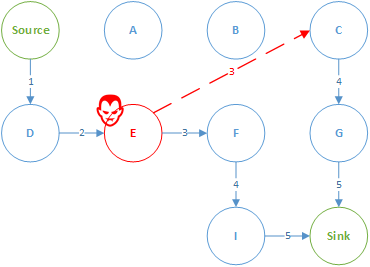
\includegraphics[width=0.8\linewidth]{figures/Directional_Antenna_Attack.png}
  \caption{Directional Antenna Attack}
  \label{fig:directional_antenna_attack}
\end{figure}

A mitigation strategy could be to analyse the route paths of a given packet that reached the sink more that one time. The last node identifier to appear duplicated before the path started to diverge would be one who then directed the packet to multiple regions, the attacker.

\paragraph{\textbf{Wormhole Attack}}
\paragraph{}
This attack can be seen as variation of the Directional Antenna Attack but with the collaboration of two or more attackers. Instead of simply forwarding the packets to arbitrary parts of the network, the attacker emulates a link between them and advertise to the network that recently formed connection. This disrupts the topology and has severe impact on routing paths since attackers can indicate that the link cost between them is very low therefore influence the forwarding decisions of neighbour nodes. By using these malicious routes, the energy consumption is increased because either this channel doesn't exist at all (packets are dropped and need to be resent), or the transmission cost between the attackers is greater than the normal message propagation through the network. Figure \ref{fig:wormhole_attack} shows an example where two vampires emulate a connection between them influencing the routing decisions of their neighbours.

\begin{figure}[h]
  \centering
  \includegraphics[width=0.8\linewidth]{figures/Wormhole_attack.png}
  \caption{Wormhole Attack}
  \label{fig:wormhole_attack}
\end{figure} 

Wormhole attacks can be prevented using the Markle tree authentication. This tree is organized from the leafs towards the root where every parent knows their children and asks them for authentication based on their ID and public key.

\subsubsection{RPL Specific Attacks}
\paragraph{} 


\paragraph{\textbf{Selective Forwarding Attack}}
\paragraph{}
In a selective forwarding attack, a malicious node can launch a \ac{DoS} attack by selectively forwarding packets. It's main goal is to disrupt routing paths but can be used to filter any protocol. For sustainability an attacker could let the RPL control messages pass by and drop the remaining packets. Depending on the routing scheme being used (source routing or stateful tables) the source could first verify path availability or each node could dynamically decide to forward the packet through another path with similar quality. In any case a good approach would be to report those failures to the underlying RPL system in order to improve the path quality.

\paragraph{\textbf{Hello Flooding Attack}}
\paragraph{}
The Hello in the name of this attack comes from the initial message a node send when joining a network. By broadcasting this message with a strong signal power, an attacker can try to introduce himself as neighbour to many nodes of the network, or at least force a large portion of the network so spend energy starting the message exchange for node insertion. A simple solution for this attack would be to test the bi-directionality of the link. If no acknowledgement is received, the path is discarded. Another approach, if geographical locations of the nodes are known, would be to discard every hello message coming from a location beyond the transmission capabilities of ordinary nodes.

\subsubsection{Protocol Independent}
\paragraph{}
The last addressed category is not dependant on network topologies or protocol messages. It focuses on attacks that can be performed regardless of the used protocol and whose goal it to obtain information about a network device. With that information an attacker can, for example, try to include himself in the network as a legitimate device or spoof his identity to forward traffic towards him. A couple examples of these attacks are the Clone and Sybil Attacks.

\paragraph{\textbf{Clone ID and Sybil Attack}}
\paragraph{}
As the name suggests, in a clone ID attack, the attacker steals the identity of a legitimate network node by copying the information of that node onto another node. This way the attacker can gain access to the traffic that was destined to the legitimate node, prevent packets to reach their intended destination and even influence voting schemes. The Sybil attack is similar to the Clone ID, with the difference that the attacker uses several stolen identities on the same physical node. This way, large parts of a network can be taken over without the need to deploy several physical nodes. Figure \ref{fig:clone_attack} shows an example of a clone ID attack where the cloned attacker received the packet that was originally destined to the legitimate node.

\begin{figure}[h]
  \centering
  \includegraphics[width=0.8\linewidth]{figures/Clone_attack.png}
  \caption{Clone ID Attack}
  \label{fig:clone_attack}
\end{figure} 

Proposed mitigation strategies for this type of attacks consist on keeping track of the number of instances of each identity. By using the node neighbours, either a centralized or distributed approach could be used to detect duplicate entries.

\subsection{Secure Bootstrapping}
\label{sec:secure_bootstrapping}
\paragraph{}
The term bootstrapping is applied to the process in which a new device is connected to an existing network. To achieve a secure bootstrapping, a unique identity and security parameters are associated with the device during this phase. There are several ways to carry out the initial setup, either via a physical interface or wirelessly. In the case of wireless bootstrapping, attention must be given to eavesdropping so that the secure credentials cannot be intercepted.\\
Since many of the studied attacks are to be performed by a malicious intruder capable of interacting with the network, if we could assure a secure bootstrapping, meaning that the new node would be authenticated before becoming an active member of the network, a large portion of those attacks could no longer be performed. The following bootstrapping techniques were summarized in \cite{Fischer2012} and aim at providing secure bootstrapping for \ac{IoT} devices.

\subsubsection{Token Based}
\paragraph{}
In token based distribution, device specific security credentials are generated and written to a token. That token can range from memory sticks or flash cards to \ac{RFID} tags or smartcards. Is has the advantage that this initial credential generation can be performed on a physically controlled environment and only later, on the commissioning phase, is the token plugged into the device. After the successful insertion of the security credentials, the token can be removed and collected back into the secure environment. This process can be considered of high security since the credentials are generated on a closed environment and are transmitted through a physical link. To further increase the security level, a password could be used to encrypt the credentials, however that would require the device to have some kind of interface that to insert the password. If the case of large number of devices, this approach would be unsuitable due to the management effort of manually deploying the tokens to the devices \cite{Fischer2012}.

\subsubsection{Identifier Based Access Control List}
\paragraph{}
With an identifier based \ac{ACL}, new devices are allowed or denied access to the network based on their unique ID. A commonly used identifier is the MAC address. This has some major drawbacks in security since, firstly, provides no assurances on the first time the device connects to the network. An attacker can easily intercept the first messages and get access to the device information. And secondly, after the bootstrapping phase, MAC addresses can be spoofed by an attacker, allowing him access to the network by bypassing the \ac{ACL} with the identifier of a legitimate node.

\subsubsection{One Time Passwords}
\paragraph{}
The use of one time passwords enhances the manual input of credentials on the device to be bootstrapped. The person responsible for the deploy of the new node should receive through a secure channel an one time password, that would then use to authenticate the node. This one time password could be used to authenticate locally generated key material (either certificate requests or generated key pair) towards the management station or root node. The achieved security level is proportional to the security of the channel used to obtain the one time password, but assuming that channel is secure so is this method. The drawback is that it forces devices to possess some kind of interface to insert the one time password.

\subsubsection{Manufacturer Installed Credentials}
\paragraph{}
So far, excluding the identifier based access control list, the intent of the studied techniques is to supply to the new device the security credentials needed to obtain access to the network, or at least provide an authentication method that allows fetching those credentials. In manufacturer installed credentials, those security credentials are deployed during the manufacturing process of the device vendor. Those credentials are typically a public/private key pair certificate bound to the identifier of the device. This certificate can be integrated into the initial load of the firmware or stored in a separate integrated circuit designed for credential storing. In the second case, this method security can be considered very high since those integrated circuits assure that the private key cannot be read from memory. This way, the new device comes shipped with the necessary security credentials not only for the bootstrapping phase but also for the normal operation phase since it does not need to fetch any additional credentials. The effort is on the root or management station that needs to import the vendor CA certificates to assure the new device credentials are trustworthy. Also the production costs increase implying an increased device cost.

\subsubsection{Proposed Solutions}
\paragraph{}
Secure bootstrapping and network admission solutions have already been proposed in past literature. However, the development and optimization of application layer protocols as well as network layer routing schemes allows for new approaches and solutions that can now fit the in the nature of \ac{IoT} devices.
Bergman et al. \cite{Bergmann2012} proposed a three-phase secure bootstrapping technique for nodes in a \ac{CoAP} network. Firstly the joining node broadcasts a request for a \ac{CSDS}, this server, once contacted by a new node takes the responsibility of key distribution. Then the system goes under a vulnerable phase where the secret is transmitted from the \ac{CSDS} onto the new device. The author propose short audible or visual feedback to the human installer when the secret is received and assume that potential eavesdroppers can not intercept this transmission. Finally, this secret is used to setup de \ac{DTLS} connection. This approach has major security drawbacks on the secret transmission phase, the authors propose limiting the radio power to a low level and disable data forwarding beyond the local network segment, but this techniques cannot assure that an attacker wont be able to intercept the transmission.\\
Oliveira et al. \cite{Oliveira2013} proposed an admission control solution for 6LoWPAN networks based on administrative approval. Each joining node would broadcast it's presence to the network, and that broadcast would be received by the administrator in the management server. Then, the administrator would grant access to that new device based on its address, and that information would be transmitted to all the devices in the network. After this phase, the device would be allowed communication as a regular member of the network by it's neighbours. This approach has the advantage of requiring no previous setup on the device before operation but is vulnerable to the attacks previously mentioned in identifier based \ac{ACL}. The authors state that work still needs to be performed in order to validate the sensor identity and leave as possibility the pre-instalment of keys on the device. 

\section{Proposed Solution}
Before attempting to develop a protocol, or solution, that meets our goals and properly addresses the problems and attacks described in the previous chapters, it is important to define the scope of our work. A common appropriate way to do so is by presenting both a scenario and architecture of the solution. The Internet of Things is currently a hot trend and this work could potentially apply and benefit a wide spectrum of applications, ranging from home environments to large enterprise networks. However, these are domains that have different requirements. A home application should be easy to setup and not require complex configurations to the user. An enterprise solution can benefit from additional administrative configurations as long as the deployment of the devices can be done quickly and easily due to their potential large number. Our work will position itself in the middle of these two domains. We are looking at a complexity and number of devices greater than a home environment but it is not our focus to provide solutions for enterprise networks and their deployment restrictions. It is our belief that a Smart Campus is an adequate scenario and can effectively demonstrate the needs targeted by our work. In the following sections we will apply the information gathered in the previous chapters to formally define what we are trying to achieve, what are the difficulties in achieving those goals and how can we overcome them. Then, a model of a campus with the proposed energy-efficient network architecture will be presented and their component roles explained. Finally, we will discuss additional improvements that are currently out of the scope of this work but can be left for future work.

\subsection{Objectives and Requirements}
\paragraph{}
One of the major concerns regarding \ac{IoT} application is the communication model. For our work, we pose as requirement that the system is power-aware and uses the minimum energy possible. Additionally, the following set of objectives is desirable to build trust and allow secure communications to take place.

\begin{itemize}
	\item Confidentiality: Without confidential message transmission, packets would flow in the network in plain text. Attackers could sniff the packets in order to obtain information, and depending on the application this could be a security breach. Even if there is no critical data being sent, privacy is still compromised.\\
	\item Integrity: Assuring message integrity means that the message was not modified between the source and its destination. Without integrity we could not rely on the received data since it could have been, intentionally or not, modified on the fly, and be providing the system wrong information.\\
	\item Authentication: The studied type of networks relies on hop-to-hop communication, meaning several nodes will take place in forwarding a packet. If they are not authenticated they could perform a wide range of attacks and disrupt the network.
\end{itemize}

\subsection{System Architecture and Message Flow}
\paragraph{}

As stated in the beginning of the chapter, we will use a Smart Campus scenario. Due to government budget cuts on education, the \ac{IST} administration was forced to cut on the number of available staff. This personnel had the responsibility of monitoring the overall conditions of the buildings and inside environment. To cope with the staff reduction, we propose a solution for the monitoring of the campus sections by deploying a wireless sensor network on each building, connected to a central management station operated by the available staff. The scenario will be based on the \ac{IST} campus model. An overview of the system and its components over the \ac{IST} blueprints can be found in Figure \ref{fig:global_architecture}. Regarding each individual component:

\begin{itemize}
	\item Numeric Nodes: Represent the network sensor nodes, the most constrained element of the network. They cooperate to build the topology and route messages hop-by-hop until the root is reached. These are fully equipped with the energy efficient protocol stack defined in Section 4.1\\
	\item Alphabetical Nodes: Represent each topology root node. They are equipped with the same stack of the numbered nodes but are more powerful, preferentially not battery powered and act as the bridge between the constrained 6LoWPAN environment and the central management station. \\
	\item Management Station: A black box model of the core components of the system. Each building reports to the central station and the staff monitors through it. A white box model will be shown in the following sections.\\
	\item Client: The system's clients can be any user with access credentials, but mostly the staff members. They can access the management station either from within the local network or from outside through the Internet.\\
\end{itemize}
 
\begin{figure}[h]
  \centering
  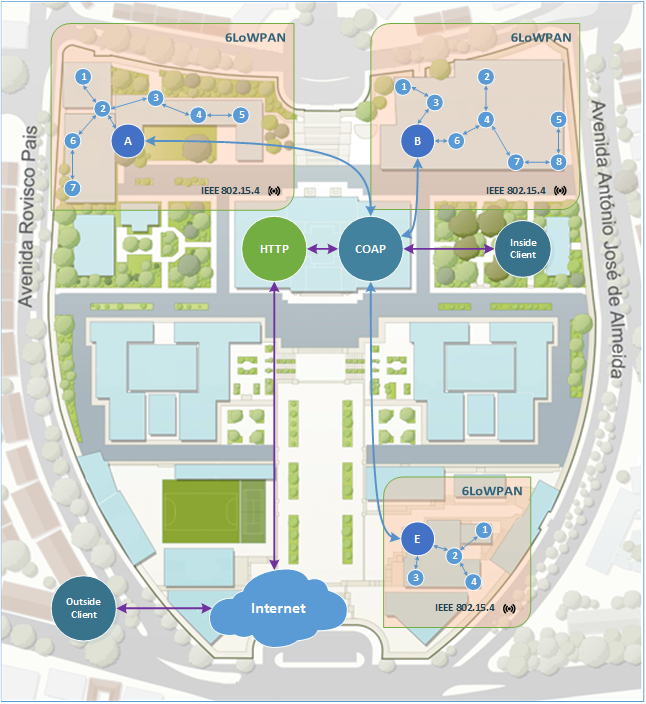
\includegraphics[width=0.8\linewidth]{figures/Global_Architecture.png}
  \caption{Global System Architecture}
  \label{fig:global_architecture}
\end{figure}

\paragraph{\textbf{Central Management Station}}
\paragraph{}

The central management station is divided in five main components. A white box schematic of the core components and interactions can be found at Figure \ref{fig:core_components}. Regarding each individual component:

\begin{itemize}
	\item Key Store: This component is responsible for storing the shared network key for the RPL protocol and a mapping between each network device and its key pair. This information is facilitated to the Client Observer for creating a secure connection to each sensor node.\\
	\item Bootstrapper: The bootstrapper acts as the interface between the management station and the network devices. It generates the device key pair and writes it together with the shared network key and the Client Observer public key into the new device.\\
	\item CoAP Client Observer:  The one and only client in the network. Instead of the user directly requesting the sensor readings, the client will observe each resource and be notified of the new value. Each time it receives an update, it stores the information on the Data Server for the clients to use.\\
	\item Data Server: A database with mappings of each node to the most up to date value reported. It's updated by the client observer and used on demand by the clients.\\
	\item Proxy: Responsible for bridging requests coming from the Internet to the Data Server. Responsible for authenticating the external clients and providing access to the Data Server information.\\
\end{itemize}

Although each user could access the system through a \ac{CoAP} terminal and request the most up-to-date readings from the sensor nodes, this approach would cause many overheads in the system. Firstly, and since many clients can connect from different locations, many requests would be performed to the sensor nodes for the same information. Additionally each sensor node would need to be pre-installed with the public keys of all the different user terminals. This would mean additional memory usage in the physical devices, and more requests to the already constrained battery operated network. With the single client approach acting as an observer, only one message needs to go through the network for each new reading.

\begin{figure}[h]
  \centering
  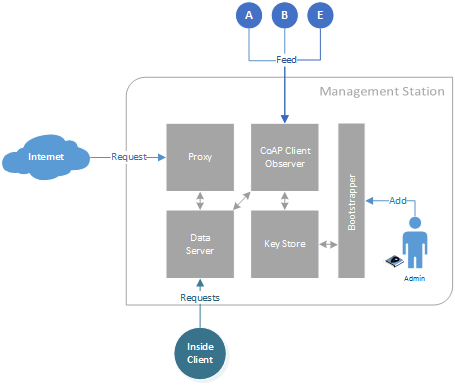
\includegraphics[width=0.8\linewidth]{figures/White_Box_Model.png}
  \caption{Central Management Station}
  \label{fig:core_components}
\end{figure}

\paragraph{\textbf{Credentials Configuration}}
\paragraph{}

In order to achieve secure communications, the new node must connect to the RPL network in a secure way, that is by using a pre shared group key. After that network setup, it will also need to make a DTLS handshake with the client observer, for that needing a key pair and the public key of the client observer. That information is written into the device during the configuration phase, done by the staff members. Figure \ref{fig:sequence_bootstrapping} shows a sequence diagram of the initial configuration phase. This process will be fully automated without requiring the staff administrator any knowledge of the inner workings of the network and authentication procedures.

\begin{figure}[h]
  \centering
  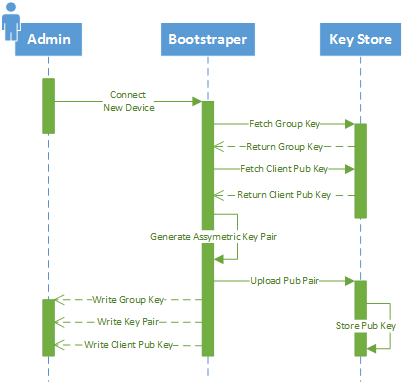
\includegraphics[width=0.8\linewidth]{figures/Sequence_Bootstrapping.png}
  \caption{New Device Initial Configuration}
  \label{fig:sequence_bootstrapping}
\end{figure}

As shown in the sequence diagram, the process is initiated by a staff member by connecting a new device to the bootstrapper. The bootstrapper automatically requests the network group key from the key store and the Client Observer public key. Then a new key pair is generated and stored in the key store for that device. Finally the bootstrapper writes the group key, the key pair and the Client Observer public key into the device.

\paragraph{\textbf{Network Layer Bootstrapping}}
\paragraph{}

After the credentials configuration phase, the new device is fully equipped with the security credentials required for joining the RPL network. Figure \ref{fig:sequence_network_admission} shows a sequence diagram of process started by the new node to join the network topology. The vocabulary used to represent the message exchange was previously presented in Section \ref{sec:network_layer}. All the message exchange is done with the secure versions of the RPL control messages, meaning the data is cyphered with the shared group key.

\begin{figure}[h]
  \centering
  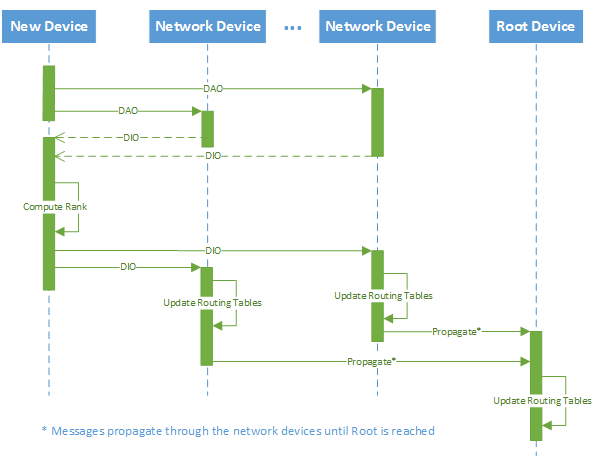
\includegraphics[width=0.8\linewidth]{figures/Sequence_Network_Admission.png}
  \caption{Network Layer Bootstrapping}
  \label{fig:sequence_network_admission}
\end{figure}

As shown in the sequence diagram, the process is initiated by the joining device by broadcasting \ac{DAO} messages to any available neighbour devices in range. The receiving nodes will reply to the new device with a \ac{DIO} message that provides graph routing information. With this information the new device is able to compute its rank (the distance towards the root) and define its parents based on that metric. After that process is complete, the new device tells his neighbours about its position in the graph using a \ac{DIO} message and the receiving nodes update their routing tables so that downwards traffic can now reach the new node. This information is further propagated up the network topology until the root is reached.

\paragraph{\textbf{Application Layer Bootstrapping}}
\paragraph{}

Although the device is now bootstrapped at the network layer, it still needs to discover and be discovered at the application layer. This means contacting the Client Observer, securing the channel through \ac{DTLS} and then send new readings as they occur. Figure \ref{fig:sequence_application_admission} shows a sequence diagram of process started by the new node to join the \ac{CoAP} network.

\begin{figure}[h]
  \centering
  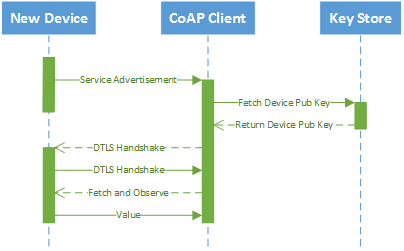
\includegraphics[width=0.8\linewidth]{figures/Sequence_Application_Admission.png}
  \caption{Application Layer Bootstrapping}
  \label{fig:sequence_application_admission}
\end{figure}

As shown in the sequence diagram the process is started by the new device that advertises its services to the network. That message is eventually received by the Client Observer who uses the new device public key, stored in the key store to start a \ac{DTLS} secured channel. After the handshake is completed, the Client Observer requests the latest readings to the sensor and sets the observe option meaning each time there is a change in the sensor reading the client will be notified.

\subsection{Limitations and Future Work}
\paragraph{}

The use of secure RPL messages with the pre-shared group key together with the raw public/private key pairs assures that a new device is properly authenticated when joining the network as well as confidentiality and integrity of the propagated packets. However, as discussed in Section \ref{sec:attack_analysis}, an attacker could try to introduce himself in the network by stealing the keys from a deployed device. The solutions for that attack can be either software based, assuring that secure memory areas cannot be copied to external locations. Or hardware based, certain integrated circuits assure the stored information cannot be read from them. This attack will not be mitigated in our system as we believe the mitigation strategies are outside the scope of this project and more related to other engineering fields of research.\\

\section{Work Evaluation}
Following the power-aware perspective of this work, our solution will evaluate the power consumption of the system in several scenarios with different network configurations:

\begin{itemize}
	\item No Security: The system does not provide any type of security credentials. All messages are exchanged in plain text and no node authentication is performed.
	\item Shared Key: The system provides to new nodes a shared group key that enabled them to join a secure instance of the network layer protocol RPL therefore assuring node authentication at the network layer.
	\item Asymmetric Cryptography : The system provides to new nodes an asymmetric key pair and the client observer public key. This enables the new nodes to join a secure instance of the application layer protocol \ac{CoAP} therefore assuring node authentication at the application layer. Moreover, this enables the \ac{DTLS} handshake to be performed using raw public keys assuring message confidentiality and integrity.
	\item Full Security Credentials: The system provides to new nodes both the shared group key, the asymmetric key pair and the client observer public key. 
\end{itemize}

After the data is collected, it will be analysed and charted so that the added power consumption of inserting security measures can be traced to the increasing power consumption. This will allow a network administrator to consider the type of device and powering mechanisms to deploy based on the security level he desires for a given application.

\section{Work Planning}
The work on the proposed solution is guided by the following schedule:

\begin{itemize}
	\item January 9\textsuperscript{th} 2016 - January 31\textsuperscript{st}: Search for the most suitable protocol and operating system implementations for constrained devices.
	\item February 1\textsuperscript{st} 2016 - February 29\textsuperscript{th}: Implementation of the proposed solution
	\item March 1\textsuperscript{st} - March 15\textsuperscript{th}: Testing and Debugging on Network Simulator
	\item March 16\textsuperscript{th} - March 31\textsuperscript{th}: Testing and Debugging on Physical Constructed Network
	\item April 1\textsuperscript{st} - April 11\textsuperscript{th}: Measure, profile and document energy consumptions for the previously described test cases.
	\item April 12\textsuperscript{th} - May 12\textsuperscript{th}: MSc Thesis Writing
	\item May 13\textsuperscript{th}: MSc Thesis Delivery
\end{itemize}

\section{Conclusion}
Due to the limitations of \ac{IoT} devices, achieving secure communications is not an easy task. In order to allow the deployment of battery powered nodes, their communication model must be very efficient and consume the minimum amount of power required for operation. To achieve those requirements we started by analysing the existing protocols across the OSI layers, trying to find the best suited solutions for this type of environments. After a thorough comparison we achieved a working stack of protocols but soon discovered possible breaches and attacks, specially on the network layer. Those attacks were further investigated and catalogued, providing an overview of the attacks spectrum. Given the common principle on the majority of the attacks, the introduction of rogue nodes to the network, we presented some possible solutions based on secure bootstrapping, the secure authentication of new nodes when joining a network.
Once the energy efficient stack, possible attacks and mitigation strategies were defined, we proposed our solution based on a Smart Campus scenario. This solution is focused on providing the joining devices all the secure credentials required for a secure bootstrapping before the deploy on the field, so that when they start the operation phase no additional credentials need to be fetched, implying that no additional energy is spent on configuration.
Always maintaining a power-aware perspective, the system will be evaluated by measuring its energy consumption with different configurations. These range from no security where messages are sent in plain text and no node authentication is performed, to full security, where the node is authenticated at network and application layers and messages are sent cyphered. This charting allows future users of the system to decide the type of resources they need to allocate in order to achieve a desired level of security for their application. As future work, currently out of the scope of this project, memory access protection should be addressed in order to the prevent the stealing of secure credentials from deployed devices.

%
% ---- Bibliography ----

\bibliographystyle{splncs}
\bibliography{references.bib}


% *** DEFINITION OF ACRONYMS ***
\acrodef{API}{Application Programming Interface}
\end{document}
